\documentclass[12pt]{article}
\usepackage{enumerate, amsmath, amsthm, amssymb,multirow}
\usepackage{graphicx}

\addtolength{\oddsidemargin}{-.5in}
\addtolength{\evensidemargin}{-.5in} \addtolength{\textwidth}{1.0in}
\begin{document}

\title{Mathematical Modeling and Optimization}

\maketitle

\section{The Problem}

You are building computers from spare parts, and you want to optimize the total value of the
computers built.  There are two types of computers that you can build: Type X and Type Y.  However,
you have limited resources, in particular only 3 monitors and 11 processors.  \\

Building one Type X computer requires 1 monitor and 5 processors, while building one Type Y computer
requires 1 monitor and 3 processors.  Type X computers are worth \$1000 each, and Type Y computers are worth
\$4000 each.  In addition, we have the additional constraint that we cannot build more than 3 Type Y computers.  
How many computers of each type should we build? \\

For this problem, assume that fractional computers are worthless, and remember that we cannot build negative computers!  

%\section{Formulation}
%
%Let $x$ and $y$ be the number of Type X and Type Y computers that you decide to build respectively.  
%
%\subsection{Objective Function}
%We are trying to maximize the total value of the computers that we build.  Because Type X and Type Y computers are
%worth \$1000 and \$4000 respectively, their total value is $1000x + 4000y$.  Therefore, the objective function is:
%\[
%\max 1000x + 4000y
%\]
%
%\subsection{Constraints}
%We need to write constraints for each of the limited resources, which are monitors and processors.
%Because Type X and Type Y computers require 1 monitor each, the total number of monitors that we use
%is $x + y$.  We only have 3 monitors, so this is an upper bound for the total number of monitors.  Therefore,
%the monitor constraint is:
%\[
%x + y \leq 3
%\]
%
%Because Type X and Type Y computers require 5 processors and 3 processors respectively, the total number of processors
%that we use is $5x + 3y$.  We only have 11 processors, so this is an upper bound for the total number of processors.  Therefore,
%the processor constraint is:
%\[
%5x + 3y \leq 11
%\]
%
%\subsection{Decision Variables}
%The decision variables are $x$ and $y$, which were defined at the beginning of this section.  Since we cannot build
%negative computers, we need to add the constraints $x \ge 0$ and $y \ge 0$.  Also, we cannot build more than 3 of the Type Y computers, so we add the constraint $y \leq 3$.  Therefore, we have:
%\[
%x \geq 0
%\]
%\[
%0 \le y \leq 3
%\]
%
%Since we do not want to build fractional computers, we add the integer constraint for $x$ and $y$:
%\[
%x, y ~\textup{integer}
%\]
%
%\subsection{Final Formulation}
%Putting all of the previous parts together, we obtain the full optimization model:
%
%\begin{equation}
%\label{eq:opt_1}
%\begin{array}{rl}
%\max~ & 1000x + 4000y \vspace{3pt}\\
%\textup{s.t.}~ & x + y \leq 3 \vspace{3pt}\\
%& 5x + 3y \leq 11 \vspace{3pt}\\
%& x \geq 0 \vspace{3pt}\\
%& 0 \le y \leq 3 \vspace{3pt}\\
%& x, y ~\textup{integer}\\
%\end{array}
%\end{equation}
%
%To check that we have covered all of the necessary constraints, read through the problem again and
%see if we have used all of the information that was given to us.  Now, we are ready to code up the
%optimization problem and solve it on the computer!  

\section{More Examples}

\subsection{Furniture Company}
You are in charge of a manufacturing plant for a furniture company that produces tables, chairs, and desks.  
In order to maximize revenue, you would like to determine the optimal number of tables, chairs, and desks to produce.  \\

Tables require 6 planks of wood, 2 hours of carpentry work, and 4 hours of machine work to produce.  Chairs require 2 planks of wood, 2 hours of carpentry work, and 2 hours of machine work to produce.  Desks require 5 planks of wood, 3 hours of carpentry work, and 6 hours of machine work to produce.  We have 500 planks of wood, 300 hours of carpentry work, and 450 hours of machine work total that we can use.  Tables sell for \$60, chairs sell for \$40, and desks sell for \$100 respectively.  \\

Assuming that we cannot build fractional products, how many pieces of each type of furniture should we produce?  Formulate this as an optimization problem, with an objective function and constraints.  

\subsection{Star Wars Assault!}
General Leia Organa is leading the Rebel Alliance space invasion of Starkiller Base, the latest superweapon designed by the First Order to annhilate planets from far away solar systems.  She needs to decide which spacecraft to send on this dangerous but critical mission, and the fate of the entire galaxy depends upon it.  

To optimize the chances of a successful mission, General Leia wants to maximize the total amount of firepower of the spacecraft.  There are 3 different types of spacecraft which may go on this mission: the X-wing starfighter, the B-62 bomber, and the JP-9 fuel jet, which have are armed with 4 blasters, 20 blasters, and 0 blasters respectively.  There are plenty of each type of spacecraft, but the Rebel alliance has a limited suppy of 12 blast shields, 60 pilots, and 8000 megaliters of rocket fuel.  The X-wing starfighter requires 1 blast shield, 1 pilot, and 200 megaliters of rocket fuel.  The B-62 bomber requires 1 blast sheild, 8 pilots, and 600 megaliters of rocket fuel respectively.  The JP-9 fuel jet requires 1 blast sheild, 4 pilots, and {\bf generates} a net total of 1200 megaliters of extra rocket fuel that can be used for other ships.  \\

How many spaceships of each type of furniture should General Leia assign to this mission?  Formulate this as an optimization problem, with an objective function and constraints.  

\begin{figure}[ht!]
\centering
    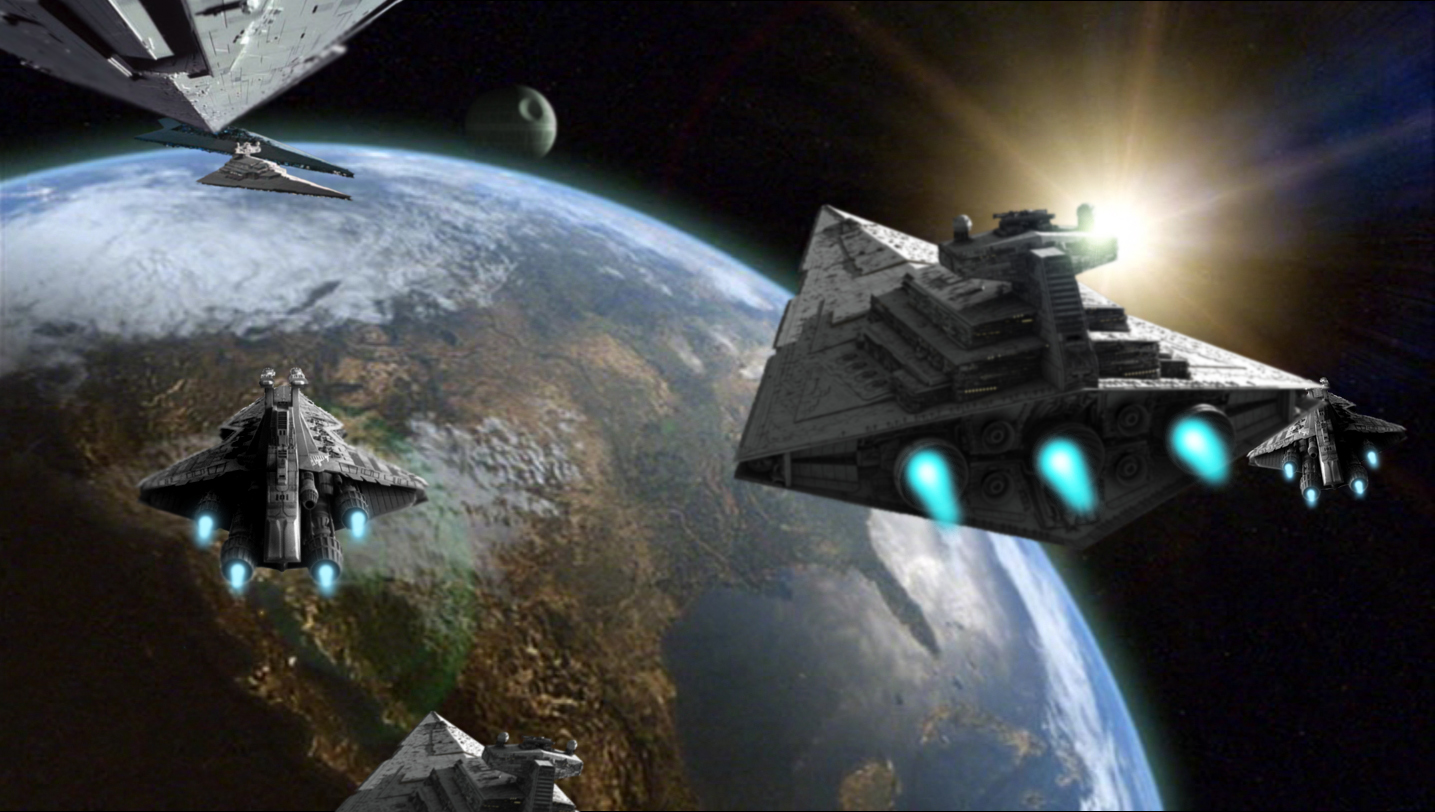
\includegraphics[width=0.8\textwidth]{pictures/Imperial_Invasion_of_Equestria}
    \caption{Star Wars Imperial Invasion of Equestria}
\end{figure}

% http://starwars.wikia.com/wiki/Leia_Organa

\subsection{New England Power}
The electricity in New England comes from a variety of sources, including nuclear, fossil-fuel, wind, and solar power plants.  
Every day, the electrical grid is optimized at the central hub, in order to meet demand while minimizing cost.  Assume for simplicity that there are only 4 power plants: A, B, C, D which have maximum output of 800, 400, 600, and 350 terawatts (TW) respectively, and we are trying to allocate power between the western and eastern halves of Massachusetts.  \\

One terawatt is 1,000 gigawatts.  Power plants A, B, C, D each have a base cost of \$2000, \$1600, \$2800, \$2200 per gigawatt respectively.  Based on the geographic location of the power plants, the transmitting cost varies.  The transmitting costs for power plants A, B, C, D are \$200, \$600, \$1200, \$100 per gigawatt for Eastern Massachusetts and \$800, \$600, \$200, \$900 per gigawatt for Western Massachusetts respectively.  The total cost is the sum of the base costs and the transmitting costs.  The demand for tomorrow is 900 terawatts in Eastern Massachusetts, and 700 terawatts in Western Massachusetts.   In addition, because power plant A is nuclear, we cannot have more than 25\% of our total power supplied by power plant A.  \\

 How many gigawatts should we allocate from each power plant to Western and Eastern Massachusetts?  Formulate this as an optimization problem, with an objective function and constraints. \\
 
(Hint: Define the decision variables $AW, BW, CW, DW$ as the amounts of gigawatts supplied to {\bf Western} Massachusetts from power plants A, B, C, D respectively.  Similarly, define the decision variables $AE, BE, CE, DE$ as the amounts of gigawatts supplied to {\bf Eastern} Massachusetts.)

\begin{figure}[ht!]
\centering
    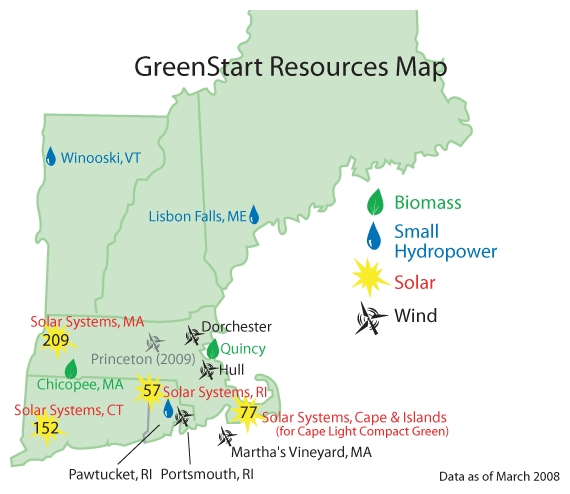
\includegraphics[width=0.8\textwidth]{pictures/resource_map_08}
        \caption{Power plants in New England region}
\end{figure}

\end{document}



